% LLNCS macro package for Springer Computer Science proceedings;
% Version 2.21 of 2022/01/12
%
\documentclass[runningheads]{llncs}
%
\usepackage[T1]{fontenc}
% T1 fonts will be used to generate the final print and online PDFs,
% so please use T1 fonts in your manuscript whenever possible.
% Other font encondings may result in incorrect characters.
%
\usepackage{graphicx}
% Used for displaying a sample figure. If possible, figure files should
% be included in EPS format.
%
% If you use the hyperref package, please uncomment the following two lines
% to display URLs in blue roman font according to Springer's eBook style:
%\usepackage{color}
%\renewcommand\UrlFont{\color{blue}\rmfamily}
%
\begin{document}
%
\title{Orchestrating information governance workloads as stateful services using Kubernetes Operator Framework}
%
%\titlerunning{Abbreviated paper title}
% If the paper title is too long for the running head, you can set
% an abbreviated paper title here
%
\author{Cataldo Mega\inst{1}\orcidID{0000-0002-2816-2699} }
%
\authorrunning{Cataldo Mega }
% First names are abbreviated in the running head.
% If there are more than two authors, 'et al.' is used.
%
\institute{University of Stuttgart, Universitätsstrasse 38, 56095 Stuttgart, Germany
\email{cataldo.mega@ipvs.uni-stuttgart.de}\\
\url{https://www.ipvs.uni-stuttgart.de/institute/team/Mega/} 
}
%  

\maketitle              % typeset the header of the contribution
%
\begin{abstract}
Regulatory compliance is forcing organizations to implement an information governance (IG) strategy, but many are struggling to evolve their IG solu-tions due to their legacy architecture, as they are not designed to adapt to new business models and for the growing amount of unstructured data pro-duced by a potentially worldwide audience. One of the biggest problems faced is continuously determining data value and the adaptation the measures to keep risks and operational costs under control. One way to solve this issue is to leverage cloud technology and find an affordable approach to migrate legacy solutions to a cloud environment. In most cases, this means de-composing monolithic applications, refactoring components and replacing outdated homegrown deployment technologies with cloud-native, automated deployment and orchestration services. Our goal is to show how operational costs can be reduced by running refactored versions of IG solutions in clouds with a minimum of human intervention. This paper highlights the steps to evolve a legacy multi-tier IG solutions from physical to containerized envi-ronments by encapsulating human operator knowledge in cloud topology and orchestration artifacts, with the goal of enabling automated deployment and operation in Kubernetes (K8s) managed execution environments.

\keywords{Information governance   \and IG workloads   \and cloud   \and stateful services.}
\end{abstract}
%
%
%
% Chap one
\section{Introduction}
Every company is subject to three basic business metrics; Value, cost and risk. They form the basis of any Enterprise Information Management (EIM) system. IG adds governance controls to information lifecycles and becomes the control authority for Information Lifecycle Governance (ILG).  ILG starts with the creation and extends to the disposition of data. Data sets in the IG context represent governance metadata needed to control how data is processed and to create an appropriate governance context derived from applicable company policies, regulations and standards through the use of Records Lifecycle Management (RLM). This means that governance records relate to the retention, security, classification, and disposition of data. In practical terms, IG consists of implementing an Information Governance Program (IGP) that helps to steer information lifecycles based on actual data value. As a result, ILG workflows through their processes implement three key activities: 1) Use of analytics to determine and maximize data value as context erodes; 2) Enforce archiving of data onto tiered storage to ensure storage cost declines as value declines; 3) Trigger disposal of obsolete data to avoid cost and eliminate risk. As a result, in addition to actual business workloads, these activities also produce typical ILG workloads that an EIM system must handle.

\subsection{Problem statement and requirements}
Today, legacy IG solutions operating in a global open market have to deal with an increasing workload caused by international regulation pushing them to its opera-tional and financial limits. The root cause of these shortcomings is a monolithic solution design and a production system running on a static IT infrastructure. These factors prevent flexibility at component level and elasticity at IT resource level, and are therefore costly to operate and maintain. One way out of this situation is to mi-grate these solutions to cloud environments and take advantage of the economies of scale where the sharing of IT resources makes it possible to minimize operational costs and optimize resource consumption through automation. Unlike traditional IT systems, clouds automate operational cost control by monitoring key performance indicators that report on cloud resource consumption, and more important make changes to the used infrastructure as necessary through dynamic provisioning and de-provisioning. 
This paper proposes steps to evolve and adapt the legacy architecture of IG solutions designed for bare metal production environments to modern cloud environments. To prove the feasibility of our approach, we implemented a prototype of an IG solution operated on a K8s managed platform using the Cloud Native Computing Foundation (CNCF) [1] promoted operator pattern.
%
\subsection{1.2	Contributions and outline of this paper}
Contribution 1: We decomposed our IG solution, reworked its legacy design, and made the necessary changes to automatically deploy and operate it in a K8s execution environment. Major focus has been put into refactoring component and deployment models and consolidating of the tier-based high availability (HA) design be-fore moving from a bare-metal to a containerized on virtualized deployment model. Contribution 2: We formalized the knowledge of human operators and implemented a resilient IG solution that models HA, disaster recovery (DR) and scale-out by incorporating infrastructure operational logic into the design and implementation of stateless and stateful cloud services running under the control of the Kubernetes (K8s) orchestra-tor.

The remainder of this paper is structured as follows: Chapter:2 presents a blue-print for IG solutions and an associated component model that we derived from a representative set of IG use cases. Some background on the benefits that the cloud offers for IG workloads is also provided. Chapter:3 discusses the fundamental aspects of topologies for deploying IG solutions and discusses traditional versus cloud-native deployment models. It also briefly discusses how K8s based workload orchestration works in the cloud. Chapter:4 presents our solution approach. Chapter:5 introduces the stateful IG repository prototype and its services. Chapter:6 details the prototype development and the system under test (SUT). Chapter:7 discusses the evaluation performed and the test results produced; Chapter:8 presents our conclusion and provides an outlook on future work.

% Chap two
\section{Background}
Today’s cloud platforms offer dynamic resource provisioning, scalability and efficiency to applications that are both containerized and virtualized - characteristics that legacy IG solutions lack. Virtualization affects physical production environments; it transforms physical infrastructure into purely virtual infrastructure through a Soft-ware Defined Infrastructure (SDI) approach. Containerization is done at the solution level by breaking down monolithic solutions into independent components that are suitable for running inside containers.
Our approach follows the concept of a composable solution that runs on top of a composable infrastructure as coined by Gartner [2]. This approach suggests that IT resources are dynamically allocated through APIs based on policies. Composable in this context means striving for fully automated IT resource lifecycle management, where application workload pattern and Service Level Agreements (SLA) trigger resource provisioning and de-provisioning events. To prove this approach, we implemented a prototype using the IBM Content Services Architecture [3] guidelines and a subset of IBM Content Management [4] family of products.

\subsection{ILG usage scenarios}
IG requirements are mainly derived from corporate policies, regulations and stand-ards. They influence the solutions design and define RLM control structures required for EIM and RLM lifecycles processes as described by the following use cases (UC):
\begin{itemize}

\item {UC1 (EIM): Collect and classify enterprise data from known sources.}
\item {UC2 (EIM): Load, store, index and secure data in enterprise repositories.}
\item {UC3 (EIM): Search, access and retrieve information from the repositories.}
\item {UC4 (RLM): Apply regulatory classification, retention, hold, disposition policies.}
\item {UC5 (RLM): Support legal cases through e-discover, aggregate and transfer case data on hold.}
\end{itemize}

\subsection{ILG workload models}
By definition, a workload is defined as a representative mix of primitive operations performed against a system, so the workloads implied by the use cases UC1 – UC5 fall into the following categories (details are discussed in Mega [5]): 
•	WL1: This workload is created by interactive users and external agents using web-requests through Https/REST issued against the IG services APIs.
•	WL2: Is an interactive- and bulk workload, using lower-level application logic performing database operations consisting of a representative mix of primitive operations: Create, Retrieve, Update, Delete and Search (CRUDS).
•	WL3: Is an interactive- and bulk workloads using low-level file system functions issued against persisted files, consisting of digital objects of any type, format and size. 
Together, use cases, workloads and real-world experience help define an IG solution and blueprint as shown in Fig. 1. ILG Solution blueprint and component. below. It consists of seven key solution components, listed as CM1 to CM7.

\noindent Displayed equations are centered and set on a separate line.
\begin{figure}
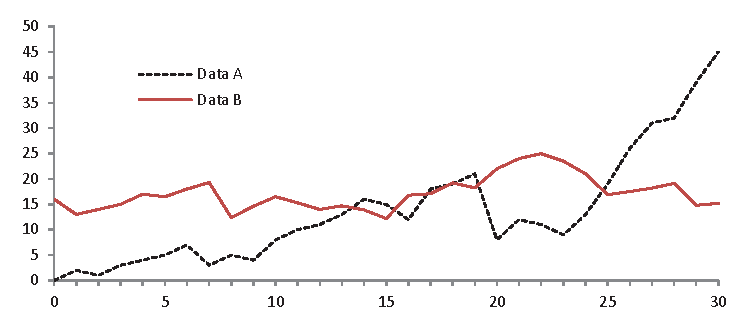
\includegraphics[width=\textwidth]{fig1.eps}
\caption{Fig. 1.} \label{fig1}
\end{figure}

The components CM1 to CM7 shown are related to, from left to right: CM1: The subcomponents Data Collection, Classification, Assessment and Ingest. CM2: Con-tent Services: Access, Index, Search, Retrieval, Security and Management. CM3: Records Services: Classification, Retention, Disposition and Compliance. CM4: Case Management Services: e-Discovery, Legal Data Requests, Holds. CM5: Con-tent Analytics: Classification, Statistics, Reporting. CM6: Repository Services: In-formation Retrieval, Catalog and Archive.  CM7: Platform Services: Compute, Stor-age, and Network. This blueprint aligns with those outlined by California Depart-ment of Technology [6], Alfresco [7], IBM Cloud Design Center [8], IBM Content Manager Enterprise Edition [4], IBM FileNet Content Manager [9], and other major players in this do-main. 
Similar, interactive, and batch workloads are discussed in Mega [5] and in Le-butsch [10], in both publications, the tests performed used a deployment topology similar to that shown in Fig.2 and the measured response time showed qualitatively similar behavior.

Fig. 2, outlines the steps from left to right, in which the IG solution on the left is broken down into individual, self-sufficient components then assembled into a de-ployment package together with the platform components and arranged as a deploy-able topology graph using a multi-tier application pattern.
\noindent Displayed equations are centered and set on a separate line.

\begin{figure}
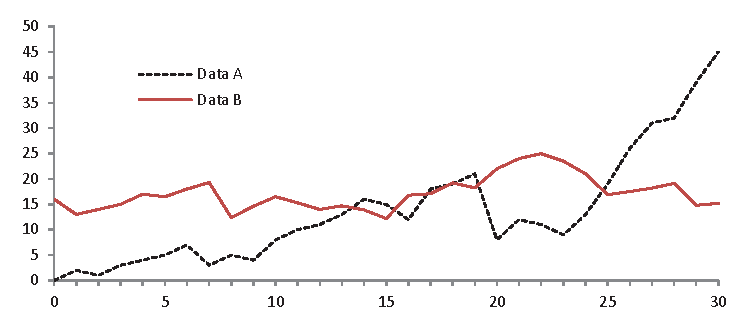
\includegraphics[width=\textwidth]{fig1.eps}
\caption{Fig. 2.} \label{fig2}
\end{figure}

% Chap three
\section{Foundation}
Before cloud, there was a gap between cluster and cluster management. The to-pology graph of Fig. 2 emphasizes this aspect were each tier is designed as a cluster of applications/resources pair configured to address the need for service resiliency and scale using component specific cluster management logic. IG solutions typically consists of multiple tiers. Examples are a web server tier, an application server tier for business logic like content repository for managing content, a database server tier for storing meta data and a storage tier to persist digital content. Service high availability mandates that every tier withstands component failure therefore a high availability solution re-quires a high availability configuration for every tier. The complexity of configuring high availability holistically stems from the fact that different tier and server types use different approaches to high availability, consist-ing of specific operational logic, to holistically maintain a defined application state and meet established service level agreements (SLA). SLAs are measured through key performance indicators like: health (alive, dead), response time and throughput. 
On clouds, cluster operations are consolidated, centralized and application agnos-tic. Cloud applications are deployed in container together with their runtime envi-ronments, in units called Pod. Pod cluster management is an integral part of the cloud platform and independent of application type. Pods are the smallest deploya-ble units in Kubernetes [11]. Cluster of Pods are centrally managed by the K8s con-trol plane, which acts as a replacement for the legacy, tier-specific cluster manage-ment. This feature is the biggest advantage for a legacy multi-tier solution. By mi-grating legacy applications from bare-metal to the cloud, it is possible to close the gap between clusters and cluster management, simplifying and consolidating the operation of an IG production system.

\subsection{ Virtualizing and componentizing a monolithic IG solution}
Fig. 3 is a visual of the platform related migration steps necessary for moving IG solutions from bare metal (left) through virtualization to containerized on virtual-ized (right) cloud execution environments, as suggested by the CNCF [1].

\begin{figure}
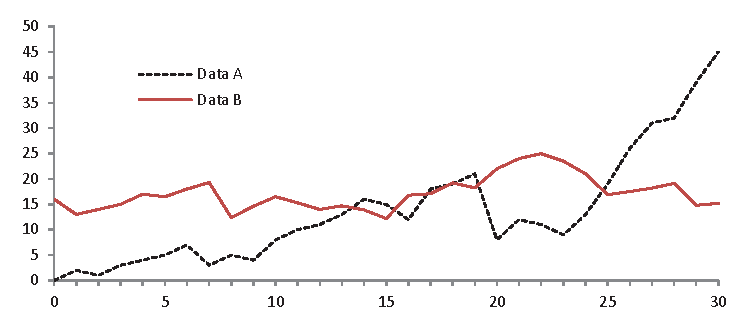
\includegraphics[width=\textwidth]{fig1.eps}
\caption{Fig. 3.} \label{fig3}
\end{figure}

As stated in our foundation, necessary condition for migrating a legacy solution is to break down monolithic applications into independent components that are suitable for running inside containers. The result is a refactored IG solution design which we used to develop our prototype. The actual migration steps performed were: 1) We decomposed the IG solution design in to smaller independent components; 2) We then virtualized the production environment, selecting OpenStack and KVM as the cloud platform/hypervisor technology (Gang [12]); 3) The third step was to contain-erize the chosen components using Docker for the container and Kubernetes for the cluster technology (Trybek [13], Hagemann [14]) for the stateless application tier components; 4) The last step included developing the stateful services based on Ku-bernetes StatefulSets and its operator frame-work (Wang [15]). Throughout devel-opment our focus was on the re-design but were possible also replacement of old components with new cloud-ready technology. As an example physical components like load balancer (LB), compute server and some networks were replaced with vir-tual resources provisioned by the cloud platform. Web  and application  tiers-specific cluster management was replaced with K8s built-in Pod cluster manage-ment. Only the management of the database cluster was custom developed by creat-ing a DB2-Operator and formalizing DB2 HA reconciliation logic through the K8s operator implementation.

\subsection{3.2	Comparing physical vs virtual infrastructure models}
Fig. 4 shows the deployment topologies of both the original physical production system versus the new virtual, cloud-based production platforms. On the left, you see the legacy system deployed on bare metal servers, in a static, pre-configured production environment. This configuration does not support dynamic topology changes of the physical resources that are provisioned manually and on request. In these environments software triggered dynamic pro(de)visioning events are not an option. 
In addition, tier specific cluster management requires more complex planning and labor intensive operator interventions. The three clusters (Cluster1-3) on the left of Fig. 4 relate to the three tiers (T1 -T3), Web, Application and Database. The right side shows the same configuration but with a K8s assisted deployment topology optimized for managing the container on virtualized infrastructure. The benefit gained is a consolidated platform built-in cluster management, including a central-ized service orchestration facility. In addition, the database specific cluster man-agement is controlled also through the K8s APIs using a custom database operator.

\begin{figure}
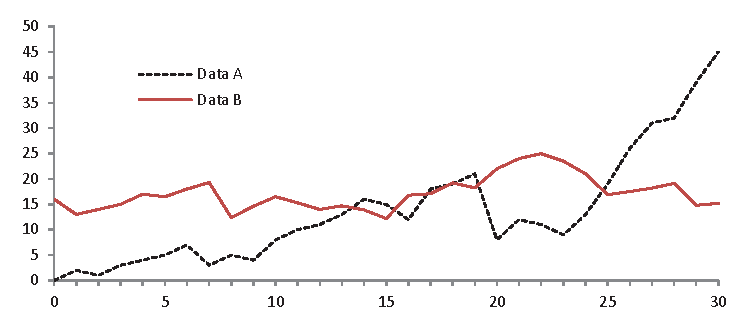
\includegraphics[width=\textwidth]{fig1.eps}
\caption{Fig. 4. Migrating solutions from physical to virtual infrastructures.} \label{fig4}
\end{figure}

\subsection{3.3	Kubernetes stateful architecture and its entities}
For a better understanding of our solutions approach, we introduce Kubernetes, its components, resources and the operator framework at the high-level. K8s key com-ponents are: Controller, Scheduler, Configuration Database (ETCD), a Node mean-ing a virtual machine (VM) and the actual Operator. The Deployment, Service and StatefulSets are K8s script resources required to define deployment topology and runtime context using YAML grammar. More specifically their definition is as fol-lows: 
•	A Deployment is a declarative description of PODs, who carry stateless services.
•	A StatefulSets  is a declarative description of PODs, carrying stateful services.
•	A Service is a declarative way to expose PODs to the external world. The Service defines network access and load-balancing policies to PODs hosting applications that provide the actual service. 
•	An Operator is a K8s extension that allows custom software to be management from within Kubernetes. This is done using a Custom Resource Definition (CRD) and the corresponding Custom Resource (CR) component via K8s APIs.
•	A Custom Resource Definition (CRD) is a declarative description representing a resource known to but not managed by K8s.
•	A Custom Resource (CR) is a component implementing a custom control loop used to manage a custom resource throughout its entire lifecycle. A CR carries the human operator knowledge in form of resource specific implementation arti-fact. 
By definition, an IG solution consists of components that provides both stateless and stateful services. This means that the following 3 K8s resources must be used to bring stateless and stateful services under the control of K8s: Deployments for state-less services; StatefulSets for modeling stateful services and operators that use ap-plication-specific management logic to control topology changes in an elastic fash-ion. Fig. 5 shows the control flow of an operator for managing the lifecycle based on state changes of a custom resource.
As previously explained, Kubernetes manages the execution environment at and above the Pod level, but not the application within the containers. The operator  pat-tern is intended to close this gap. That is, human operator functions were made available to a K8s operator to manage sets of services in an automated way via K8s APIs. For example, the imitation of a human database operator through database-specific administration logic implemented with scripts or program modules that specify setup, configuration and management of the database in a production envi-ronment.

\begin{figure}
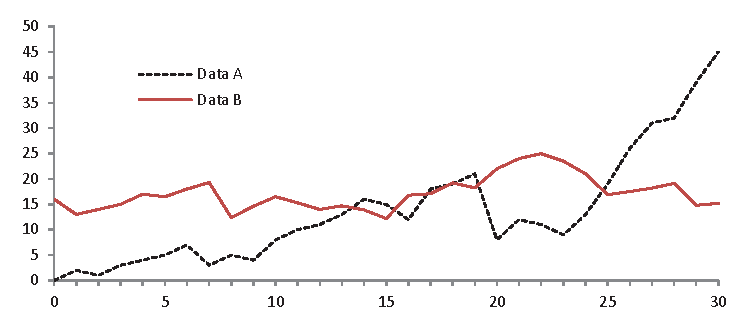
\includegraphics[width=\textwidth]{fig1.eps}
\caption{Fig. 5. K8s control loop of the operator pattern.} \label{fig5}
\end{figure}

% Chap Four
\section{Solution Approach}
For our IG solution design, we envisioned a 2-level hierarchy of five K8s operators. The first operator on the left of Fig. 6 represents the top level ILG service operator, who controls and monitors the four operators at the 2nd-level. These are the Reposi-tory service, the Client service, the ObjServer service, and the DB service, which together form the four-tiered deployment topology shown in Fig. 4. As can be seen, the web and application tiers are mapped to three stateless services implemented as K8s Deployments. The combined database and storage tier are implemented through a K8s StatefulSet, which is used to control and manage the DB service operator, as shown in Fig. 6. The DB service operator contains the definition of the DB cluster and the logic required to support high availability, read-scalability and disaster re-covery. 

We deployed and tested the prototype implementation in 2 phases. In the first phase, we focused on the stateless services of the web and application tier, which are shown as the upper part of the topology graph in Fig. 7. In the second phase, we developed and deployed the underlying stateful repository services, including the database and storage tiers shown in the image at the bottom of the topology graph. By stateful database services we mean a service that is resilience to component failures, in our context this might be database instance, a storage or a network failure. The proposed solution is to create a shared-nothing database cluster with at least 3 independent database instances and replication mechanism that replicates the database data using synchronous or asynchronous replication.
This papers focuses on the aspect of highly available stateful database services and the required orchestration logic used derived from database product guidelines and our own expertise.

\begin{figure}
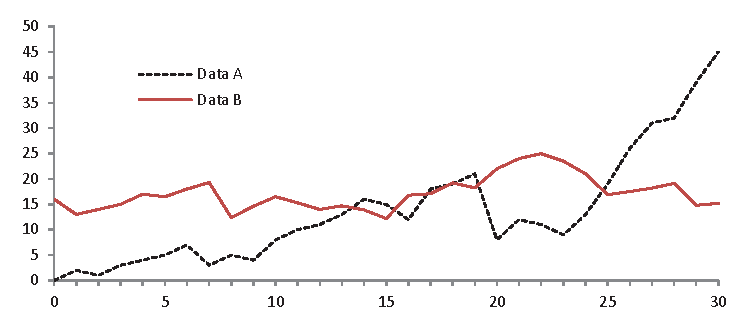
\includegraphics[width=\textwidth]{fig1.eps}
\caption{Fig. 6. K8s operator hierarchy for managing ILG deployment topology.} \label{fig6}
\end{figure}

\subsection{4.1	K8s operator extended control loop}
To support a stateful database service running a cluster of database instances in con-tainers on a virtualized in environment, it was necessary to develop database-specific cluster management using the component and a topology as shown in Fig. 7. It also shows how the integration of the database cluster and its execution environ-ment is controlled by the StatefulSet complemented by the DB2 operator, together they control the database state and topology through the K8s control plane. The DB2 operator and respective custom control loop is shown in the lower left part of Fig. 7. 
The picture shows the K8s and the DB2 control loops as so-called MAPE loops, a concept that is being discussed in Maurer [16]. MAPE stands for Monitor, Analyze, Plan and Execute, basically the chain of processes that represent the decision logic that decides which activities must follow after a change of the desired state of the stateful service. The MAPE process steps are: Monitor the target resource state; Analyze and compare current state with the desired state; Plan what to do in case misalignments of state; Execute the reconciliation plan taking the necessary actions to align current state with desired service state.

\begin{figure}
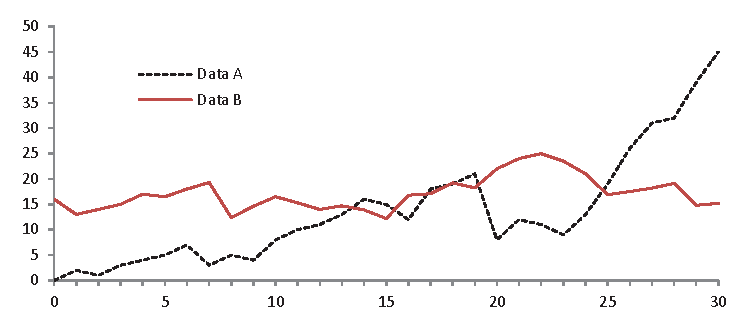
\includegraphics[width=\textwidth]{fig1.eps}
\caption{Fig. 7. ILG solution deployment topology and the K8s control loops.} \label{fig7}
\end{figure}

\subsection{4.2	Related work}
The prototype implementation work was done in the course of 4 master thesis at the university of Stuttgart by Gang [12], Trybek [13], Hagemann [14] and Wang [15]. The concept design around dynamic topology published by Mega [5], Börner [17], contribution for the integration of the MAPE loop concept came from Ritter [18]. A concept model of an EIM system including governance services was provided by the IBM Cloud Architecture Center [8]. The CNCF [1] published white paper on the Operator pattern provided the ground work for our migration approach. Andrikopou-los [19] in his paper outlines a generic introduction on how to adapt applications for the cloud. Kubernetes best practices, specific to StatefulSets and opera-tors came from Palak [20]. Aspects of EIM practices in companies from Chaki [21] motivated our work for developing migration strategies to move legacy solutions into the cloud. The California Department of Technology [6] provided most of the insight of an ECM reference architecture. The latter was complemented by information man-agement governance guidelines from other government agencies like Victoria State Government [22]. Maurer et al [16] elaborated on MAPE for autonomic manage-ment of cloud infrastructures. Our research lead to several academic sources on stateful services on cloud, but none specifically ad-dressing the aspect of refactoring legacy IG solutions and how to move them onto cloud execution platforms.

% Chap Five
\section{The ILG Repository stateful service prototype}
Compared to stateless services, stateful services are more complex to design and to implement in K8s because it was initially designed for stateless services, and stateful services were later introduced for custom resource integrating. For the prototype we chose an IG solution based on IBM ECM [4] and needed other necessary components, consisting of IBM Content Navigator, IBM Content Manager, IBM Web-Sphere Application Server and the IBM DB2 database server. This decision was based on our experience in building ECM production systems that provide information governance services, a knowledge we have acquired through several custom-er projects. The configuration of the prototype is designed to test scale, service availability and disaster recovery and translates into a set of K8s stateful services. The DB2 service operator is used specifically to automate the database cluster management through K8s APIs.

\subsection{5.1	Kubernetes stateful services cluster setup}

% Chap Six
\section{DB2-Operator prototype test system setup}
\subsection{A Subsection Sample}
\paragraph{Sample Heading (Fourth Level)}

% Chap Seven
\section{7	Tests, results and evaluation}

\subsection{7.1	Service availability and fail-over scenario}
\paragraph{Sample Heading (Fourth Level)}

\noindent Displayed equations are centered and set on a separate line.
\begin{figure}
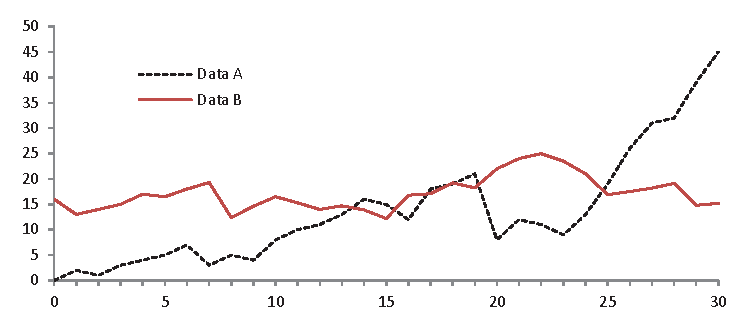
\includegraphics[width=\textwidth]{fig1.eps}
\caption{Fig. 12.} \label{fig12}
\end{figure}


Table~\ref{tab1} gives a summary of all heading levels.
\begin{table}
\caption{Table captions should be placed above the
tables.}\label{tab1}
\begin{tabular}{|l|l|l|}
\hline
Heading level &  Example & Font size and style\\
\hline
Title (centered) &  {\Large\bfseries Lecture Notes} & 14 point, bold\\
1st-level heading &  {\large\bfseries 1 Introduction} & 12 point, bold\\
2nd-level heading & {\bfseries 2.1 Printing Area} & 10 point, bold\\
3rd-level heading & {\bfseries Run-in Heading in Bold.} Text follows & 10 point, bold\\
4th-level heading & {\itshape Lowest Level Heading.} Text follows & 10 point, italic\\
\hline
\end{tabular}
\end{table}

\noindent Displayed equations are centered and set on a separate line.
\begin{figure}
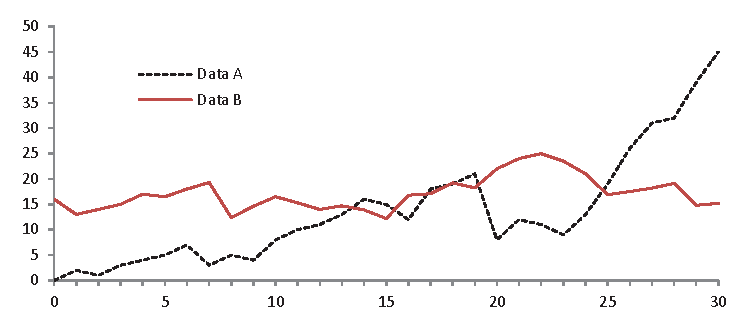
\includegraphics[width=\textwidth]{fig1.eps}
\caption{Fig. 13.} \label{fig13}
\end{figure}


% Chap Eight
\section{Conclusions and Outlook}
This paper explored the effort required to migrate a legacy IG solution designed to operate in a pre-configured, physical production environment to a dynamic software-defined cloud infrastructure (SDI). The focus of this work was on refactoring the legacy solution design and successfully moving from a physical to a cloud environment. The benefit gained from this is the ability to orchestrate ILG workloads using stateful services in K8s managed clusters. We have learned that cloud platforms provide cluster control mechanisms and resource topology management across all solution tiers, which can simplify and reduce the application-specific cluster management complexity. With a cluster managed by K8s, Pod, Node, Network and Storage management is kept out of application responsibility and centrally consolidated in the cloud platform. This makes application layer-specific cluster management obsolete and solution design leaner. In addition, built-in control loops with the cloud platform enable monitoring of resource health and automatic triggering of provisioning and de-provisioning requests. Component specific lifecycle management tasks are integrated as K8s extensions using the operator pattern. Operators makes it possible to take advantage of the elasticity of the cloud infrastructure and react dynamically to changes in workload. The resulting effects are the avoidance of manual interventions, gain in flexibility and the reduction of associated operating costs. 
Our prototype leverages the IBM ECM product stack, consisting of IBM Content Navigator, IBM Content Manager Enterprise Edition, along with the required IBM WebSphere Application Server and IBM DB2 database server. We have developed an IG solution design as used by traditional ECM customers world-wide, most of whom still run their systems on-premise on a physical infrastructure. Currently, all products support virtualized environments, but not all support containerized in virtualized environments. We could not, find a customer story that holistically shows the migration of an IG solution from physical to cloud, but several blogs explaining cloud implementations of individual component. 
Future work could focus on real-world production deployments and repeat our tests with more realistic workloads and database sizes.


%
% the environments 'definition', 'lemma', 'proposition', 'corollary',
% 'remark', and 'example' are defined in the LLNCS documentclass as well.
%
articles~\cite{ref_article1}, an LNCS chapter~\cite{ref_lncs1}, a
book~\cite{ref_book1}, proceedings without editors~\cite{ref_proc1},
and a homepage~\cite{ref_url1}. Multiple citations are grouped
\cite{ref_article1,ref_lncs1,ref_book1},
\cite{ref_article1,ref_book1,ref_proc1,ref_url1}.

\subsubsection{Acknowledgements} Please place your acknowledgments at
the end of the paper, preceded by an unnumbered run-in heading (i.e.
3rd-level heading).

%
% ---- Bibliography ----
%
% BibTeX users should specify bibliography style 'splncs04'.
% References will then be sorted and formatted in the correct style.
%
% \bibliographystyle{splncs04}
% \bibliography{mybibliography}
%
\begin{thebibliography}{8}
\bibitem{ref_article1}
Author, F.: Article title. Journal \textbf{2}(5), 99--110 (2016)

\bibitem{ref_lncs1}
Author, F., Author, S.: Title of a proceedings paper. In: Editor,
F., Editor, S. (eds.) CONFERENCE 2016, LNCS, vol. 9999, pp. 1--13.
Springer, Heidelberg (2016). \doi{10.10007/1234567890}

\bibitem{ref_book1}
Author, F., Author, S., Author, T.: Book title. 2nd edn. Publisher,
Location (1999)

\bibitem{ref_proc1}
Author, A.-B.: Contribution title. In: 9th International Proceedings
on Proceedings, pp. 1--2. Publisher, Location (2010)

\bibitem{ref_url1}
LNCS Homepage, \url{http://www.springer.com/lncs}. Last accessed 4
Oct 2017
\end{thebibliography}
\end{document}
